\chapter{Artificial Neural Networks}

Artificial Neural Networks (NN) are just another model to perform \textbf{supervised} ML: as for every other method, we look for a hypothesis map $h$ in a hypothesis space $\mathcal{H}$ that minimizes the loss over the training set (ERM). What makes them special is the hypothesis space: it can include \textbf{highly non-linear functions}, so it is very flexible. With enough neurons, a network with a single hidden layer can approximate any continuous function as closely as we want (universal approximation theorem). In networking, NNs are used for traffic classification, anomaly detection, QoS and throughput prediction, and traffic forecasting.

\section{Structure of an Artificial Neuron}
The elementary unit of a NN is the \textbf{artificial neuron}:
\begin{itemize}
    \item on the left there are the \textbf{inputs}, in general the features $x_1, \dots, x_n$ of a data point;
    \item on the right there is the \textbf{output};
    \item the inputs are connected to the neuron from left to right: $x_1$ is multiplied by the weight $w_1$, $x_2$ by $w_2$, and so on until $x_n$. These \textbf{weights are parameters} of the model;
    \item the neuron in the middle combines the weighted inputs with a weighted sum and passes the result to a function called \textbf{activation function} $\sigma$.
\end{itemize}
In formulas, the neuron computes
\[
z = w_1x_1 + w_2x_2 + \dots + w_nx_n + \mu, \qquad \widehat{y} = \sigma(z) .
\]
The weighted sum $z$ says how strongly the neuron is stimulated by the inputs: a large positive weight means that the corresponding feature pushes $z$ up, a negative weight that it pushes $z$ down. The activation function $\sigma$, if defined, transforms $z$ into the output $\widehat{y}$. The additional \textbf{offset} $\mu$ (also called bias) shifts the weighted sum; it is the same as adding a new input that is always equal to 1, with weight $\mu$, i.e. adding $\mu \cdot 1$.

\begin{figure}[h]
    \centering
    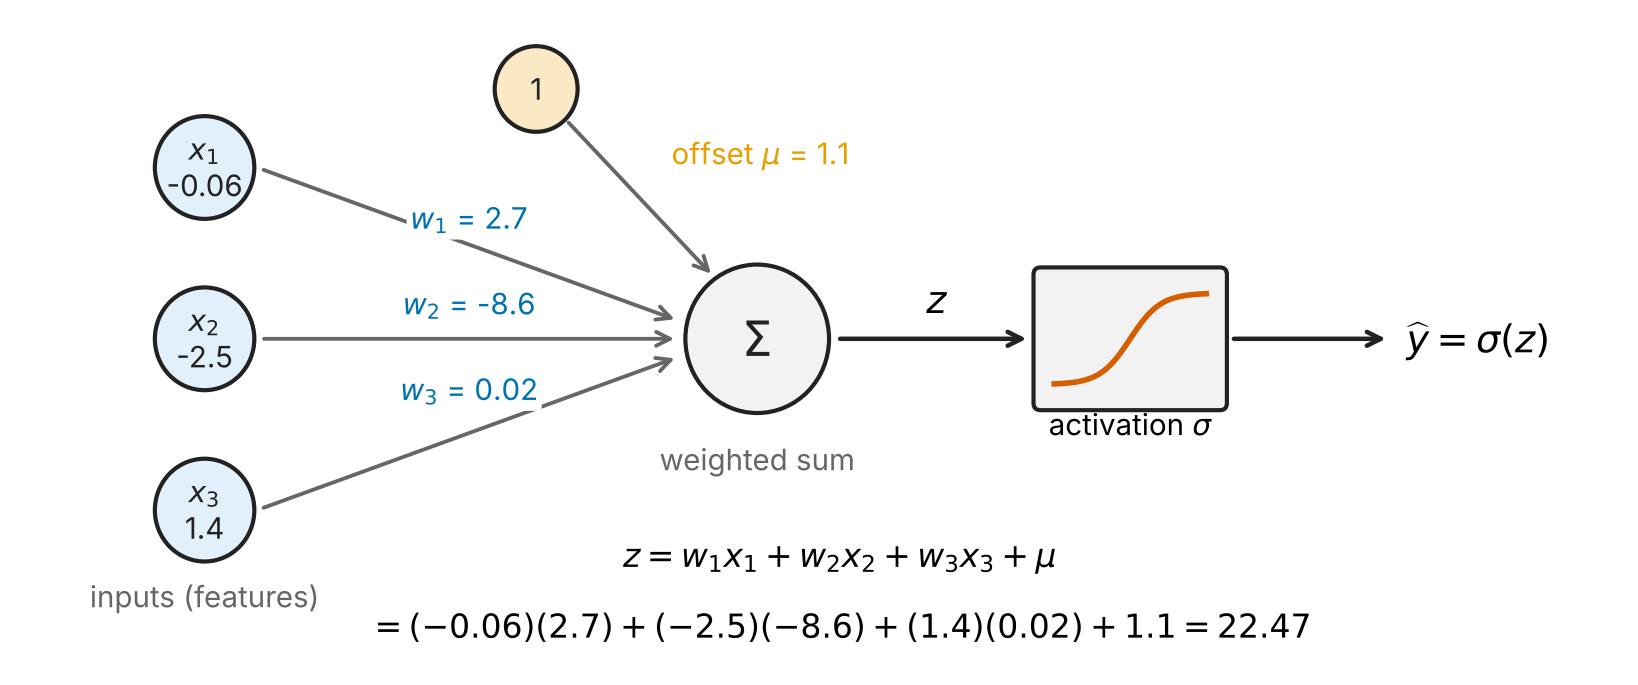
\includegraphics[width=0.95\textwidth]{images/chapter_11/neuron.png}
    \caption{An artificial neuron with three inputs, three weights, an offset and an activation function. The numbers are those of the example in the text.}
\end{figure}

For example, with inputs $x_1 = -0.06$, $x_2 = -2.5$, $x_3 = 1.4$, weights $w_1 = 2.7$, $w_2 = -8.6$, $w_3 = 0.02$ and offset $\mu = 1.1$, the weighted sum is $z = -0.162 + 21.5 + 0.028 + 1.1 = 22.47$.\footnote{Correction: the example on the slides reports $22.44$; the exact value of $(-0.06)(2.7) + (-2.5)(-8.6) + (1.4)(0.02) + 1.1$ is $22.466 \approx 22.47$.} Without activation function the output is $22.47$; with a sigmoid it would be $\sigma(22.47) \approx 1$.

A single neuron with the identity as activation (i.e. no activation) computes a linear map, so it is exactly the model of \textbf{linear regression}. A single neuron with the sigmoid activation $\sigma(z) = 1/(1 + e^{-z})$ outputs a number between 0 and 1, which can be read as the probability of class 1: this is \textbf{logistic regression}.

\section{NN as Stacked Elementary Units}
In a NN we stack many of these elementary units. All neurons compute the same kind of function, but each one has its own weights: the same feature $x_1$ enters every neuron of the next layer, each time multiplied by a different weight. The neurons are organized in layers, and the outputs of one layer are the inputs of the next one. These networks are called \textbf{feed-forward neural networks} or \textbf{multilayer perceptrons} (MLP):
\begin{itemize}
    \item the \textbf{input layer} receives the input vector, i.e. the features of the data point;
    \item the \textbf{hidden layers} are internal to the model: their values are not part of the data, we only observe the input and the output;\footnote{Clarification: the previous version said ``Hidden Layer, just internal to model. Since in our model we just need input and output''. The layers are called hidden because their values do not appear in the training data, which only contain the features (input) and the labels (output).}
    \item the \textbf{output layer} produces the output vector, i.e. the prediction.
\end{itemize}
When every neuron of a layer is connected to every neuron of the next one, the layers are called \textbf{dense} (or fully connected) layers.

\begin{figure}[h]
    \centering
    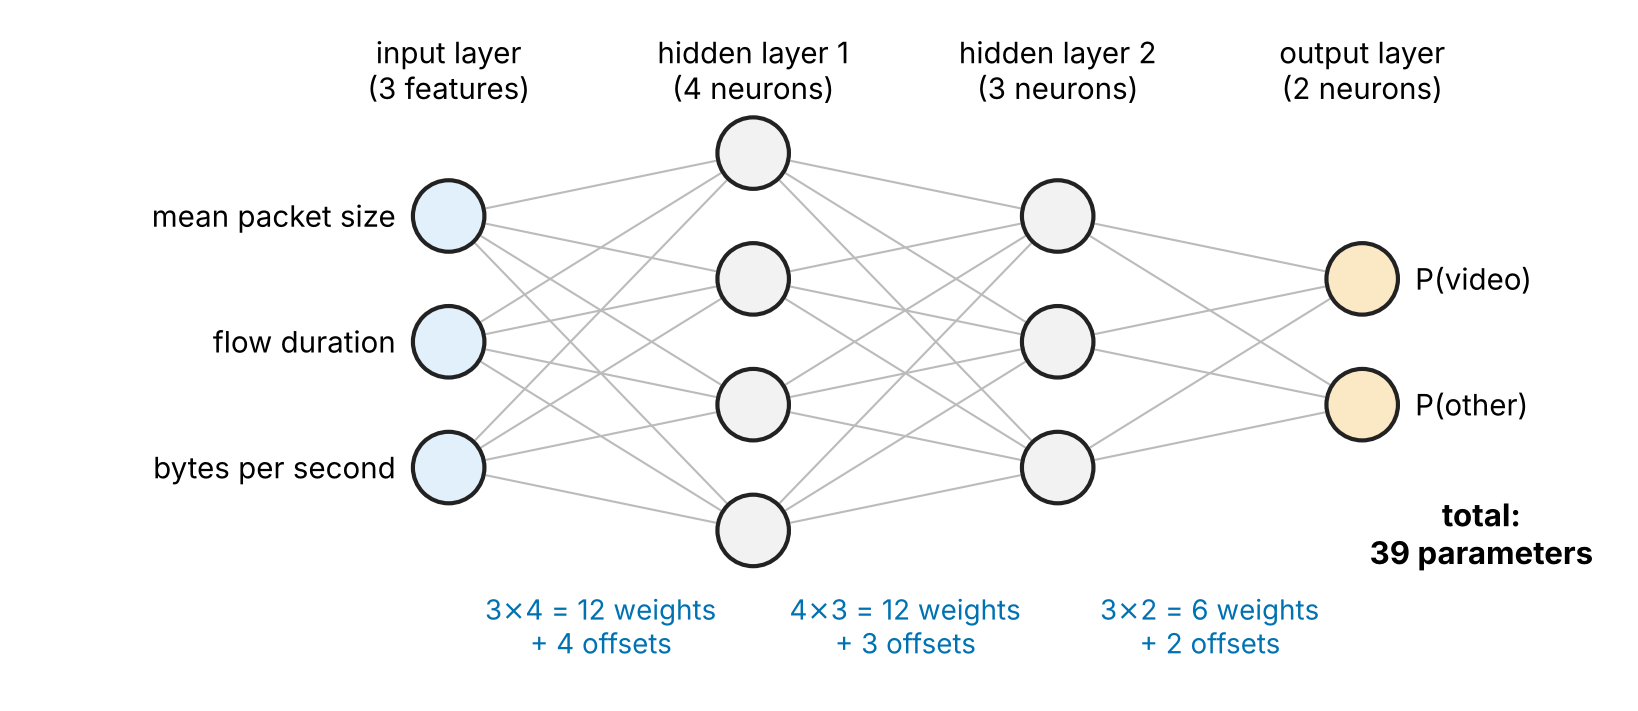
\includegraphics[width=1\textwidth]{images/chapter_11/mlp.png}
    \caption{A feed-forward network with dense layers that classifies a flow from three features. Each grey line is a weight; each hidden and output neuron also has an offset.}
\end{figure}

The number of neurons in the input and output layers is given by the problem: one input neuron per feature, and one output neuron per predicted quantity (e.g. per class). In the hidden layers, instead, we have complete freedom on:
\begin{itemize}
    \item the number of neurons;
    \item the number of hidden layers.
\end{itemize}
Therefore, we can stack as many elementary units as we prefer in the hidden layers. A specific hypothesis $h$ is obtained by fixing the weights of every connection (synapse) and the offset of every neuron.

Why does stacking simple units give such flexible functions? The figure below shows a network with one input (the utilization of a link), one hidden layer of 7 neurons with the ReLU activation $\max(0, z)$, and one output neuron without activation. Each hidden neuron produces a ``hinge'': zero up to a certain point, then a straight line. The output neuron adds the hinges with its weights, and their sum is a curve made of straight pieces, which can follow the queueing delay of the link with a maximum error of 0.35 ms. More neurons give more pieces and a closer approximation.

\begin{figure}[h]
    \centering
    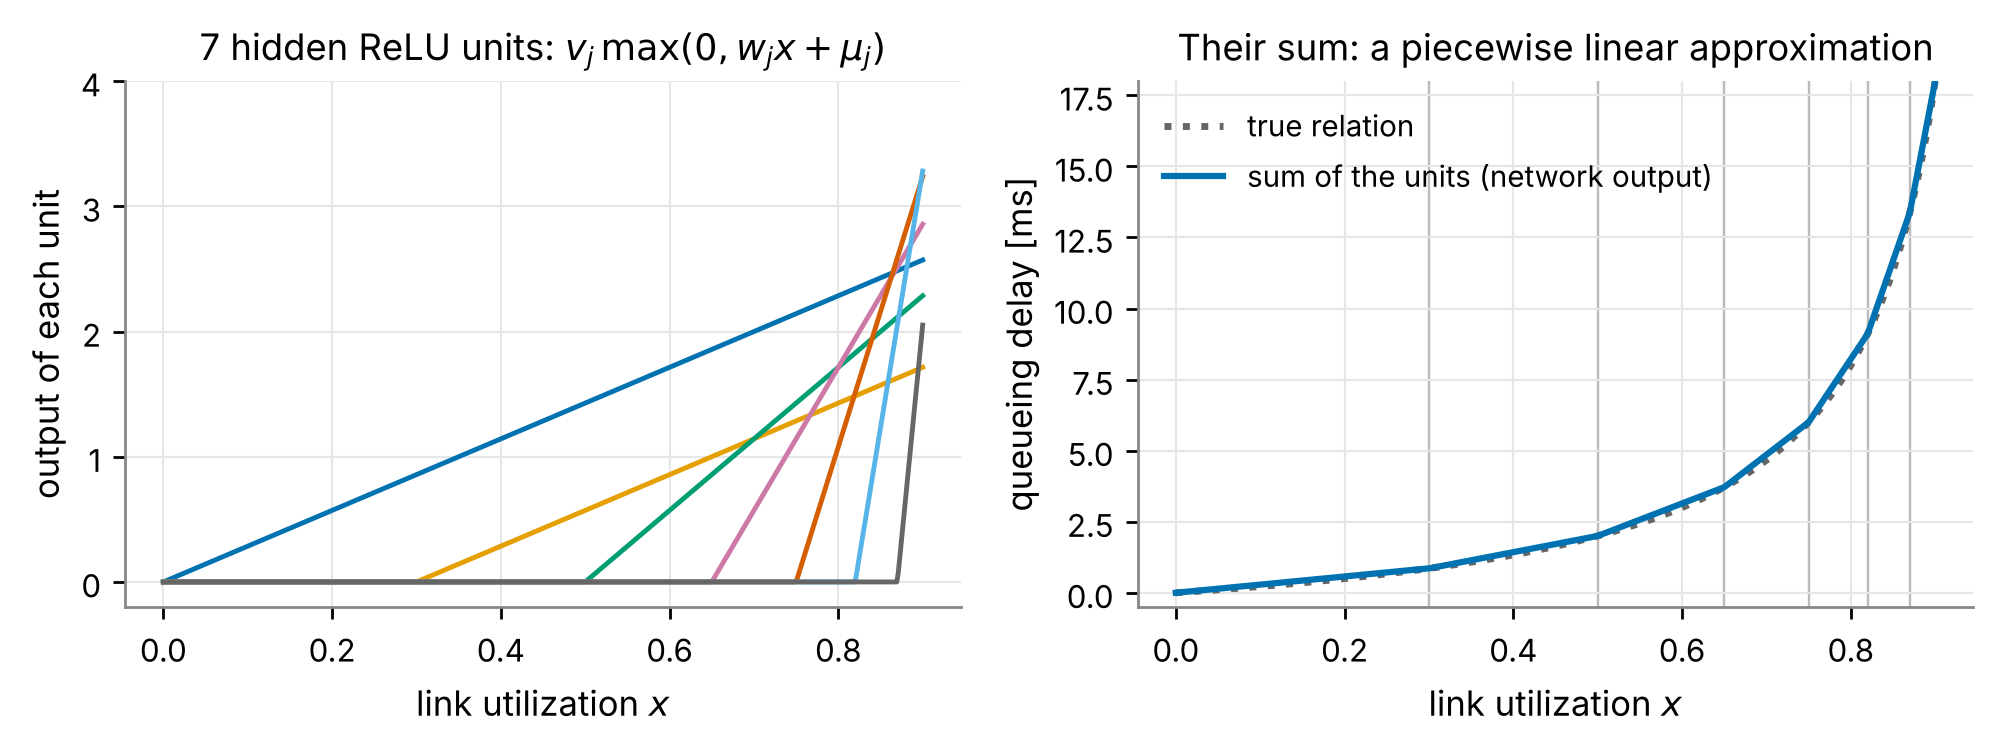
\includegraphics[width=1\textwidth]{images/chapter_11/relu_sum.png}
    \caption{Left: the outputs of 7 hidden ReLU neurons, each with its own weight and offset. Right: their weighted sum, the output of the network, approximates the queueing delay of a link.}
\end{figure}

\section{Hyperparameters of NN}
The hyperparameters that define the model, i.e. the hypothesis space $\mathcal{H}$, are:
\begin{itemize}
    \item the number of layers;
    \item the number of neurons in each layer;
    \item the activation functions of the neurons.
\end{itemize}
Hyperparameter tuning is done as usual, with a validation curve or a grid search (see the chapter on metrics and hyperparameter tuning). What defines the hypothesis, instead, are the \textbf{weights and offsets}, which are learnt automatically by ERM. There is one weight for each connection (synapse) and, if offsets are used, one offset for each neuron of the hidden and output layers; the input nodes only pass on the features and have no offset.\footnote{Correction: the previous version said that the total number of parameters is ``number of synapses + number of neurons''. The input nodes do not compute anything and have no offset, so the offsets are as many as the neurons of the hidden and output layers.} Hence
\[
\#\,\text{parameters} = \#\,\text{connections} + \#\,\text{hidden and output neurons}.
\]
For the network of the MLP figure (3 inputs, hidden layers of 4 and 3 neurons, 2 outputs) this gives $(3 \cdot 4 + 4 \cdot 3 + 3 \cdot 2) + (4 + 3 + 2) = 30 + 9 = 39$ parameters. Real networks easily have millions of parameters, which is why they need a lot of data.

\section{Training a NN}
Given a model $\mathcal{H}$, how do we find a good hypothesis $h$? We must find, for each neuron, the best set of weights and the best offset, i.e. the parameter vector $\mathbf{w}$ that minimizes the empirical risk. The empirical risk of a NN is differentiable but not convex, and no formula gives its minimum, so it is minimized with \textbf{gradient descent} (see the chapter on gradient learning), with a special way of computing the gradient, \textbf{back-propagation}.

\subsection{Forward and Backward Pass}
Each step of the training has two phases:
\begin{itemize}
    \item \textbf{forward pass}: the features of a data point go through the network, layer by layer, until the output; the prediction is compared with the true label through the loss function. If the loss is small, the weights are good; if it is large, they must be changed;
    \item \textbf{backward pass}: the gradient of the loss with respect to every weight is computed with the \textbf{chain rule}, starting from the last layer and moving back to the first one (back-propagation of the error). Then every weight is changed with a gradient descent step, in the direction that reduces the loss.
\end{itemize}

\begin{center}
\fbox{\parbox{0.9\textwidth}{
\textbf{Algorithm: training a NN with gradient descent}
\begin{enumerate}
    \item Initialize the weights and offsets with random values.
    \item \textbf{Forward pass}: for the training instances (one at a time, in mini-batches, or all of them), compute the output of each neuron, layer by layer, until the output layer; compare the output $\widehat{y}$ with the label $y$ and compute the loss.
    \item \textbf{Backward pass}: back-propagate the error, computing the gradient of the loss from the last layer to the first one.
    \item \textbf{Update} every weight and offset with a (stochastic) gradient descent step.
    \item Go back to step 2, until the loss is below a given threshold or the maximum number of epochs is reached.
\end{enumerate}}}
\end{center}
The loss is computed \emph{once}, at the output, by comparing the prediction with the label; what is computed for every neuron is the gradient of this loss with respect to its weights.\footnote{Correction: the previous version said to ``compute loss for each different neuron''. There is a single loss, computed at the output of the network; the backward pass then distributes its gradient to all the neurons.}

\begin{figure}[h]
    \centering
    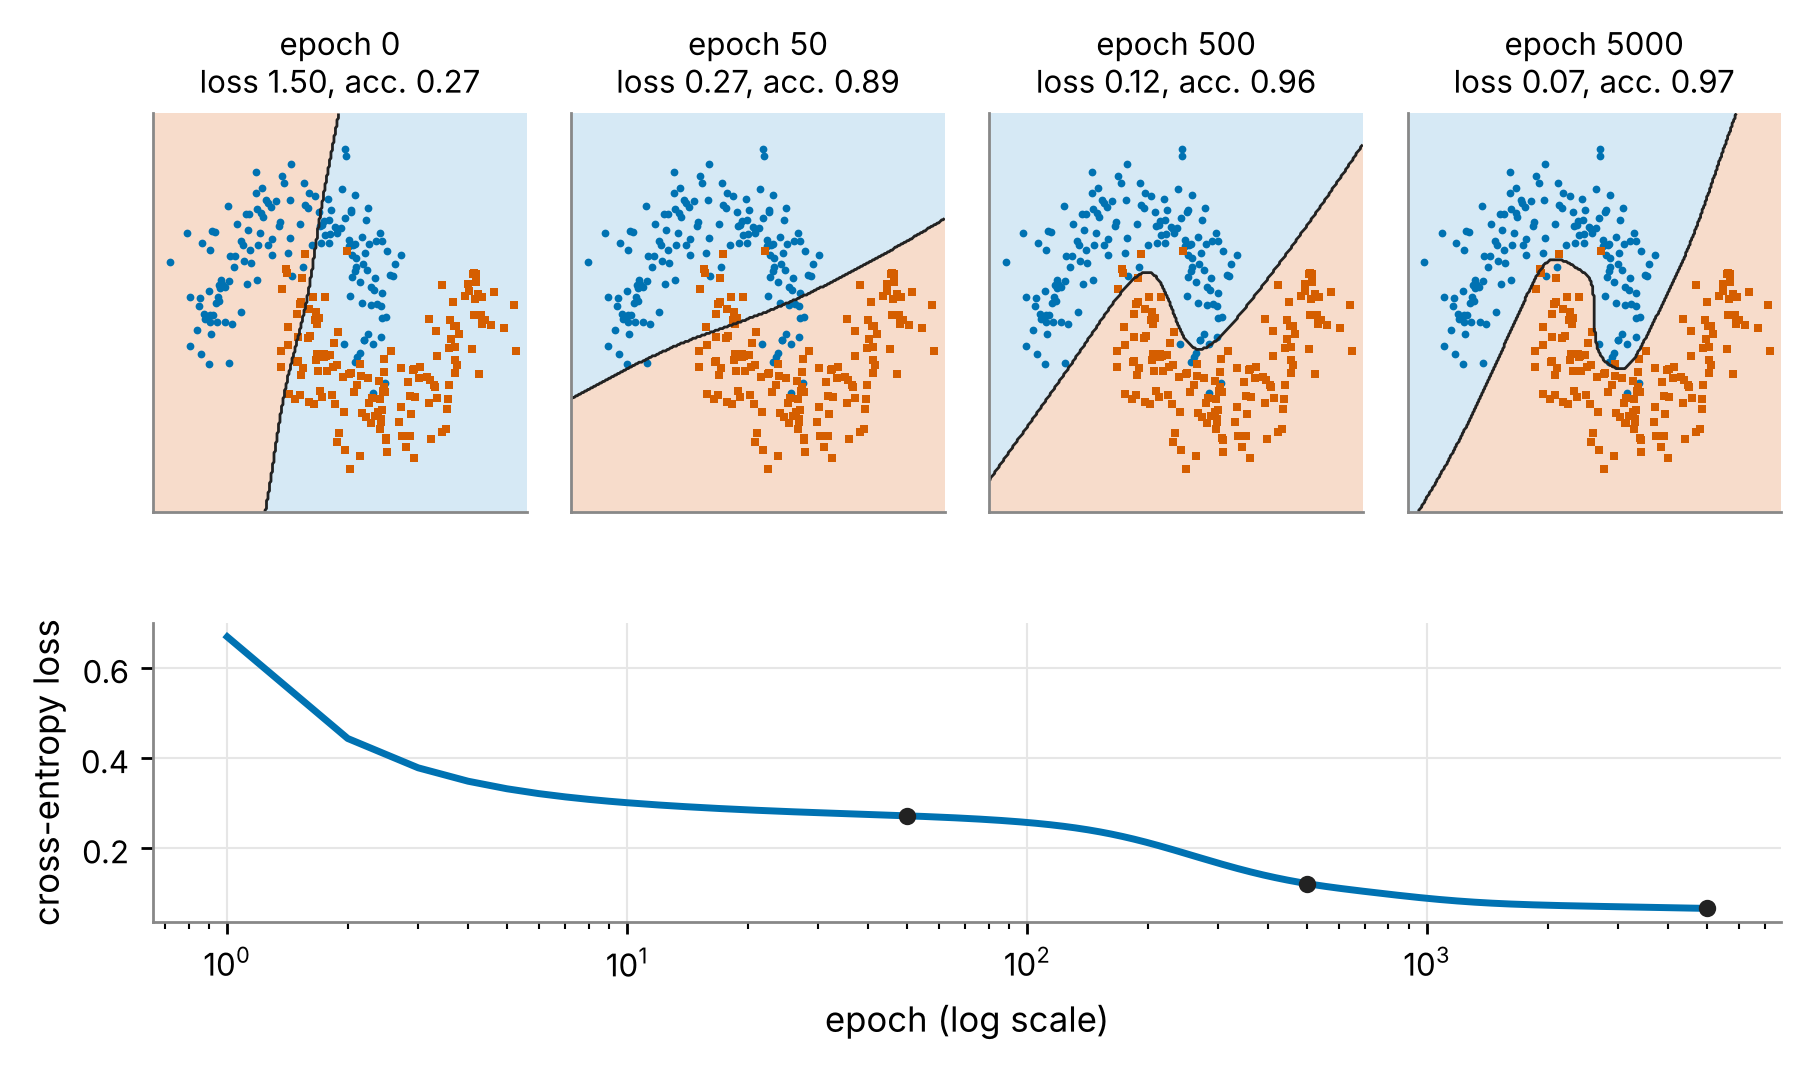
\includegraphics[width=1\textwidth]{images/chapter_11/training_evolution.png}
    \caption{A network with one hidden layer of 10 neurons (tanh) and a sigmoid output, trained with gradient descent on two interleaved classes. Top: decision boundary after 0, 50, 500 and 5000 epochs. Bottom: cross-entropy loss.}
\end{figure}

Assigning random weights in a binary classification problem gives a random decision boundary: in the figure, at epoch 0 only 27\% of the points are classified correctly. At each iteration the backward pass changes the weights so that the loss decreases, and the decision boundary improves: after 50 epochs it is a tilted line (accuracy 0.89), after 500 it starts to bend (0.96), and after 5000 it follows the shape of the two classes (0.97). Eventually, the network solves the ERM problem; since the loss is not convex, it may also stop in a local minimum.

\subsection{The Gradient Descent Step and the Chain Rule}
Each gradient descent step finds out how to change each specific weight in order to reduce the loss. Consider the simplest case, a single neuron with one input $x$, weight $w$, no offset and sigmoid activation, trained with the binary cross-entropy loss (defined in the section on loss functions). The forward pass computes three quantities, one after the other:
\[
z = wx, \qquad g = \sigma(z) = \frac{1}{1 + e^{-z}}, \qquad L = -y\ln g - (1-y)\ln(1-g) .
\]
The loss depends on $w$ only through $g$, which depends on $w$ only through $z$. The chain rule says that the derivative of $L$ with respect to $w$ is the product of the local derivatives along this chain:
\[
\frac{\partial L}{\partial w} = \frac{\partial L}{\partial g}\cdot\frac{\partial g}{\partial z}\cdot\frac{\partial z}{\partial w}
= \Big(-\frac{y}{g} + \frac{1-y}{1-g}\Big) \cdot g(1-g) \cdot x = (g - y)\,x .
\]
The sigmoid has the convenient derivative $\sigma'(z) = g(1-g)$, and after the simplification the gradient has a very intuitive form: it is the \textbf{error} $g - y$ of the prediction times the input $x$. The weight is then updated with the gradient step $w^{(r+1)} = w^{(r)} - \alpha\,\partial L/\partial w$.

\begin{figure}[h]
    \centering
    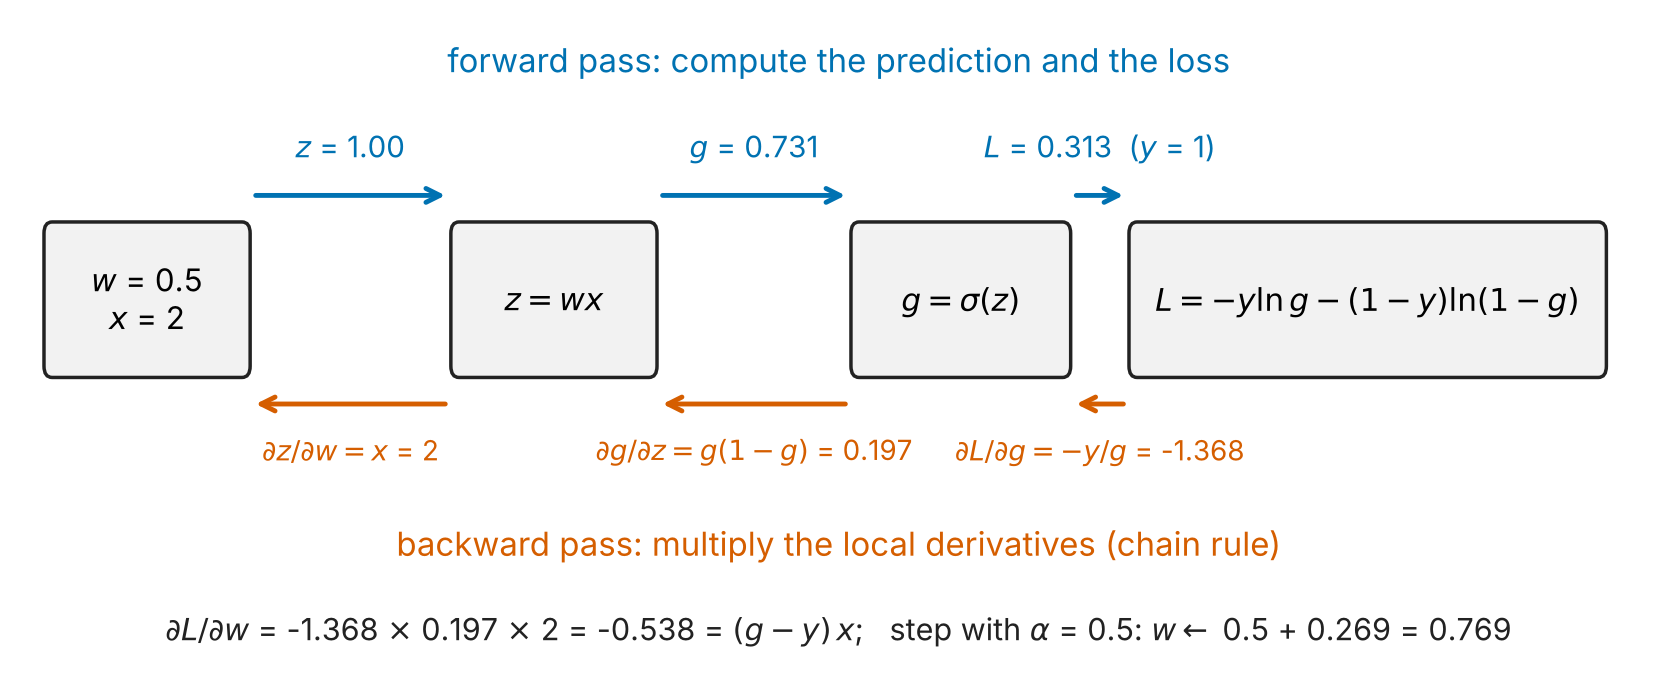
\includegraphics[width=1\textwidth]{images/chapter_11/backprop.png}
    \caption{Forward pass (top) and backward pass (bottom) for one sigmoid neuron with $x = 2$, $w = 0.5$ and true label $y = 1$.}
\end{figure}

For example, with $x = 2$, $w = 0.5$ and $y = 1$: the forward pass gives $z = 1$, $g = \sigma(1) = 0.731$ and $L = -\ln 0.731 = 0.313$. The backward pass gives $\partial L/\partial w = (0.731 - 1) \cdot 2 = -0.538$. With $\alpha = 0.5$ the new weight is $w = 0.5 - 0.5 \cdot (-0.538) = 0.769$, and indeed the loss decreases: now $z = 1.538$, $g = 0.823$ and $L = 0.195$.

This is for a single weight. With many layers, the chain rule is applied again and again, from the last layer to the first one: the gradient with respect to a weight of an early layer is the product of the local derivatives along all the paths that lead from that weight to the loss. Back-propagation organizes this computation so that each local derivative is computed only once, which makes the backward pass about as expensive as the forward pass.

\textbf{Mini-batch gradient descent} applies the step on a small random batch of training data instead of the whole training set. The gradient computed on a batch is a slightly different function from the gradient of the empirical risk, but on average it points in the same direction, so the result is similar and each step is much cheaper (see stochastic gradient descent in the chapter on gradient learning).

\subsection{Hyperparameters of Gradient Descent}
Besides the hyperparameters of the model, training has its own:
\begin{itemize}
    \item \textbf{learning rate} $\alpha$ (step size): how much the weights are changed at each step; it multiplies the gradient in the update from the current guess to the new guess. Too small and training is slow, too large and the loss oscillates or diverges;
    \item \textbf{number of epochs}: an epoch is one complete pass over the training set; with mini-batches of $B$ points, one epoch contains $m/B$ updates of the weights;\footnote{Correction: the previous version defined epochs as ``how many times we update model's weight''. An epoch is a full pass over the training set; the number of weight updates in one epoch is $m/B$ with mini-batches of size $B$, and is 1 only for plain (full-batch) gradient descent.}
    \item \textbf{batch size} $B$ of stochastic gradient descent: the number of training points used to compute each gradient;
    \item the \textbf{version of the optimizer}: plain (stochastic) gradient descent or one of its variants, e.g. with momentum or with an adaptive learning rate per weight (Adam).
\end{itemize}
For example, with $m = 10\,000$ flows and $B = 100$, one epoch consists of 100 gradient steps, and 20 epochs of 2000 steps.

\subsection{Activation Functions}
Activation functions:
\begin{itemize}
    \item simulate the biological activation of a neuron in response to input stimuli;
    \item provide \textbf{non-linearity} to the computation;
    \item help to saturate the outputs in \textbf{fixed ranges}, e.g. between 0 and 1.
\end{itemize}

\paragraph{What happens if there is no activation function?} Each layer then computes a linear map of its inputs, and a linear map of a linear map is still a linear map. In the end, the overall behaviour of the NN is always a linear map: the NN returns a linear predictor, whatever the values of the weights and offsets and however many layers it has. It is the \emph{non-linear} activation applied after each weighted sum that breaks this chain and makes the output a non-linear function of the inputs.\footnote{Correction: the previous version said ``If we add a linear function, the output of weighted sum is still linear but then passing through activation function the output can be not anymore linear''. The weighted sum is always linear; the output becomes non-linear only if the activation function is non-linear (a linear activation would keep the whole network linear).}

\begin{figure}[h]
    \centering
    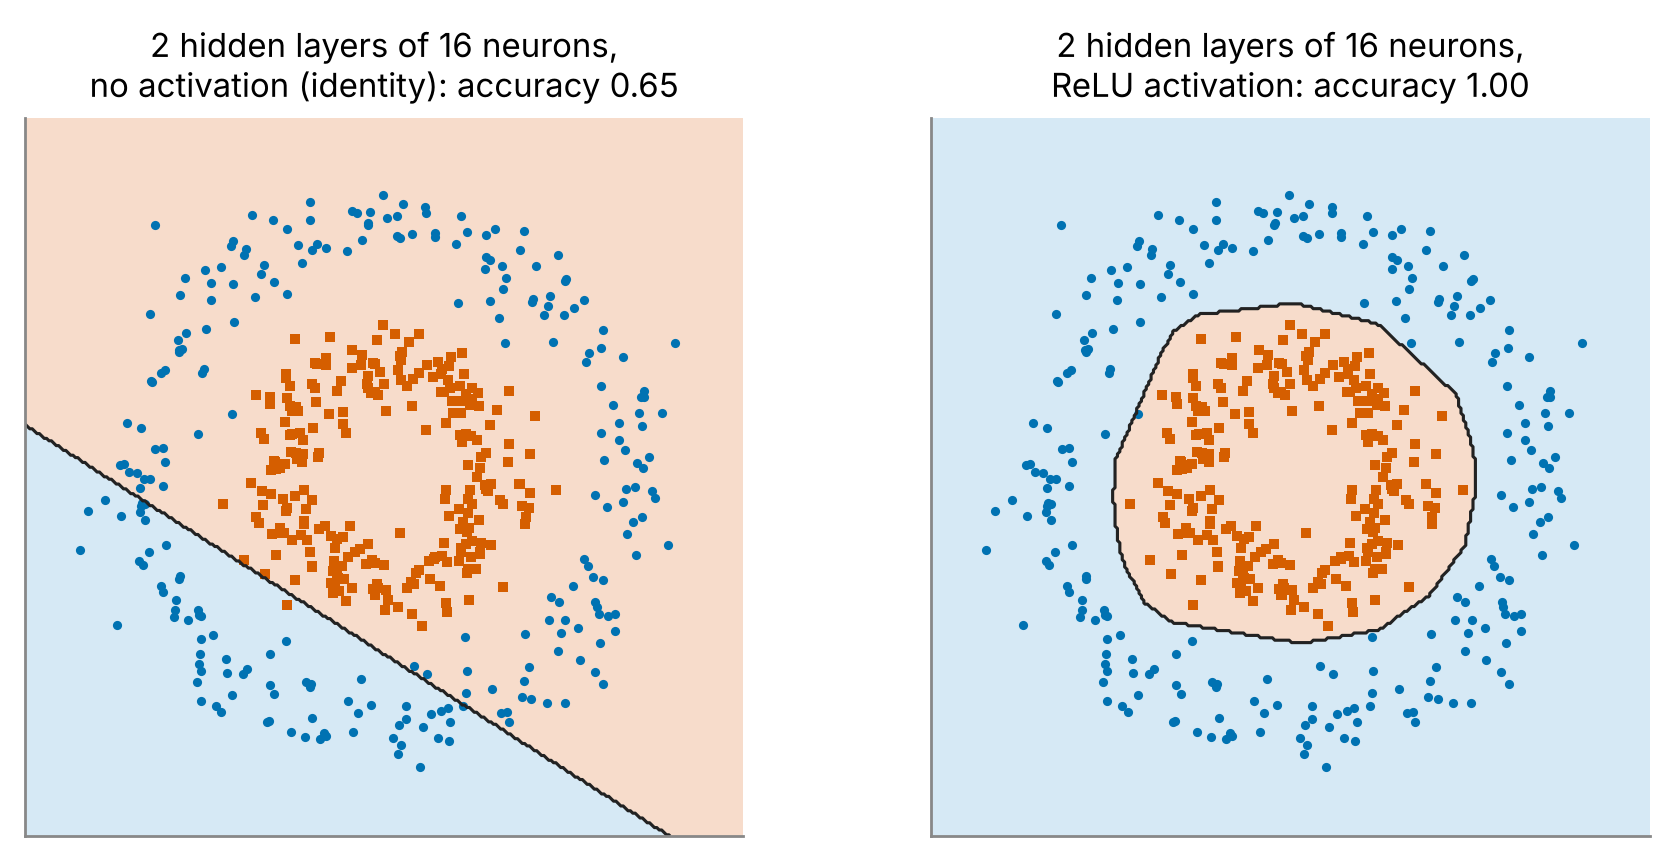
\includegraphics[width=0.85\textwidth]{images/chapter_11/linear_vs_nonlinear.png}
    \caption{The same architecture (two hidden layers of 16 neurons) trained on two concentric classes. Without activation it can only draw a straight line; with ReLU it separates the classes.}
\end{figure}

\paragraph{Examples of activation functions.}
\begin{itemize}
    \item \textbf{Sigmoid} $\sigma(z) = 1/(1 + e^{-z})$: output between 0 and 1, interpreted as a probability.
    \item \textbf{Tanh} $\tanh(z)$: output between $-1$ and $1$, centred at 0.
    \item \textbf{Binary step}: 1 if $z \geq 0$, 0 otherwise. Useful for a binary output, but not appropriate for gradient methods: its derivative is 0 everywhere (and undefined at 0), so it gives no direction for the update.
    \item \textbf{ReLU} $\max(0, z)$: zero for negative inputs, the identity for positive ones. It is cheap to compute and its derivative is 1 for every positive input, so the gradient does not vanish through many layers; it is the default choice for hidden layers.
    \item \textbf{Softmax}: an activation function for a whole layer, not for each single neuron as the previous ones.\footnote{Correction: the previous version said ``activation function for whole layer, not for each layer as before''. The previous activation functions are applied to each neuron separately.} It is usually applied to the output layer, and it works by considering all the neurons of the layer together:
    \[
    \text{softmax}(z_j) = \frac{e^{z_j}}{\sum_{i=1}^{N} e^{z_i}} ,
    \]
    where $z_j$ is the weighted sum of the $j$-th of the $N$ neurons of the layer. The outputs are between 0 and 1 and sum to 1, so the output vector can be interpreted as a discrete probability distribution: the probability that the input belongs to each class. The output of each neuron depends on the outputs of all the others: if one score grows, all the other probabilities decrease. The softmax generalizes the sigmoid to more than two classes.
\end{itemize}

\begin{figure}[h]
    \centering
    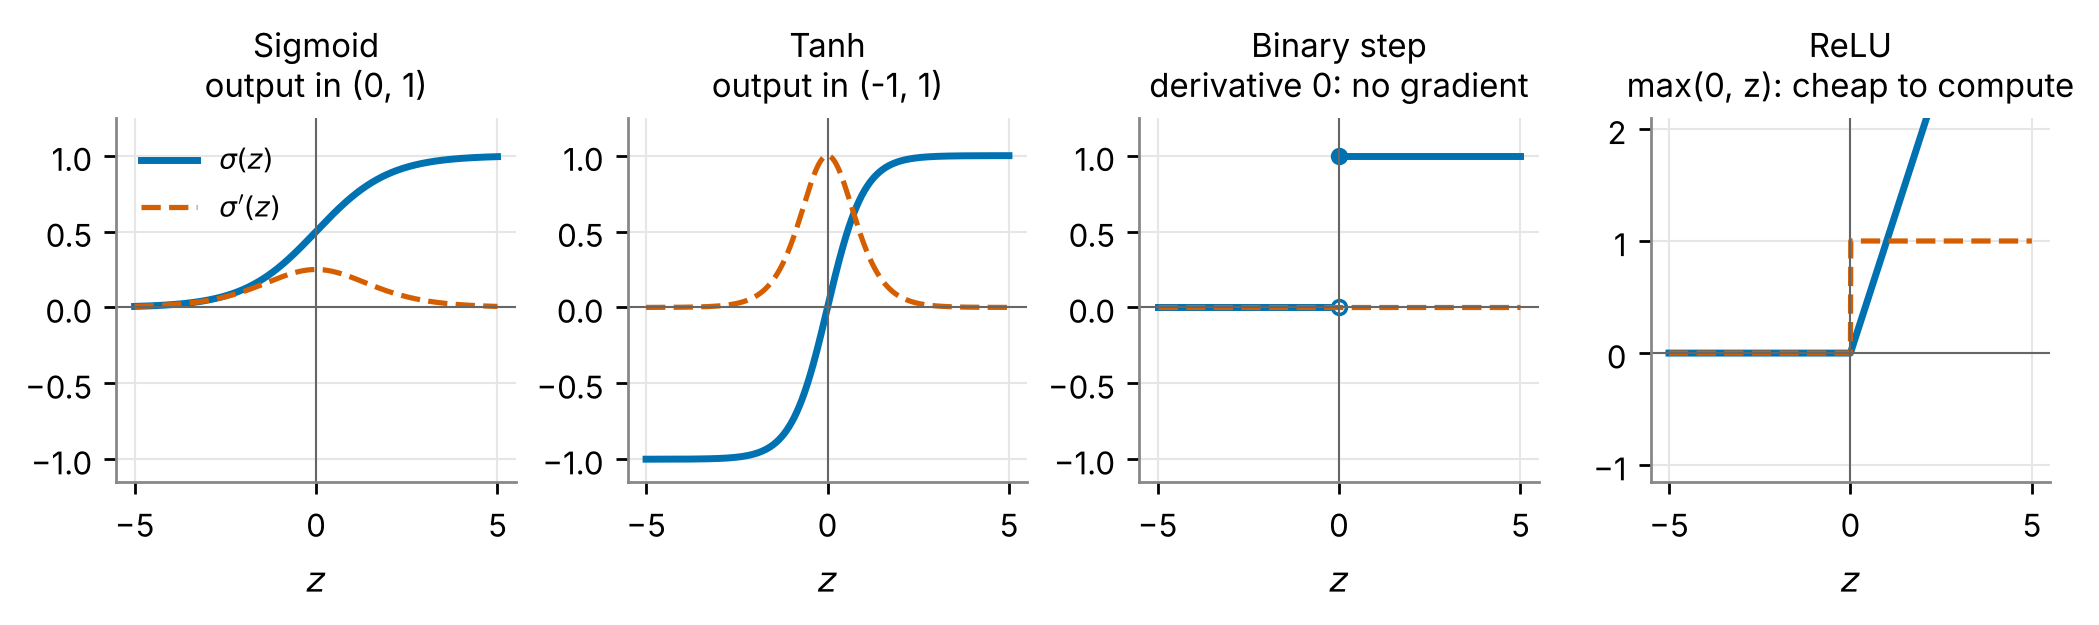
\includegraphics[width=1\textwidth]{images/chapter_11/activations.png}
    \caption{Activation functions (solid) and their derivatives (dashed), which drive the gradient descent updates.}
\end{figure}

The activation of the \textbf{output layer} depends on the task:
\begin{center}
    \begin{tabular}{l|c|l|l}
        \textbf{Task} & \textbf{Outputs} & \textbf{Activation} & \textbf{Loss} \\ \hline
        Regression            & 1   & none           & squared error \\
        Binary classification & 1   & sigmoid        & binary CE \\
        Multi-class           & $k$ & softmax        & categorical CE \\
        Multi-label           & $k$ & sigmoid (each) & binary CE per label \\
    \end{tabular}
\end{center}
Here CE stands for cross-entropy and $k$ is the number of classes or labels. For a binary output we use the sigmoid with one output neuron; for a multi-class problem, the softmax; for a multi-label problem, a sigmoid on each output neuron, because each label is a separate yes/no question and the probabilities need not sum to 1.

\begin{figure}[h]
    \centering
    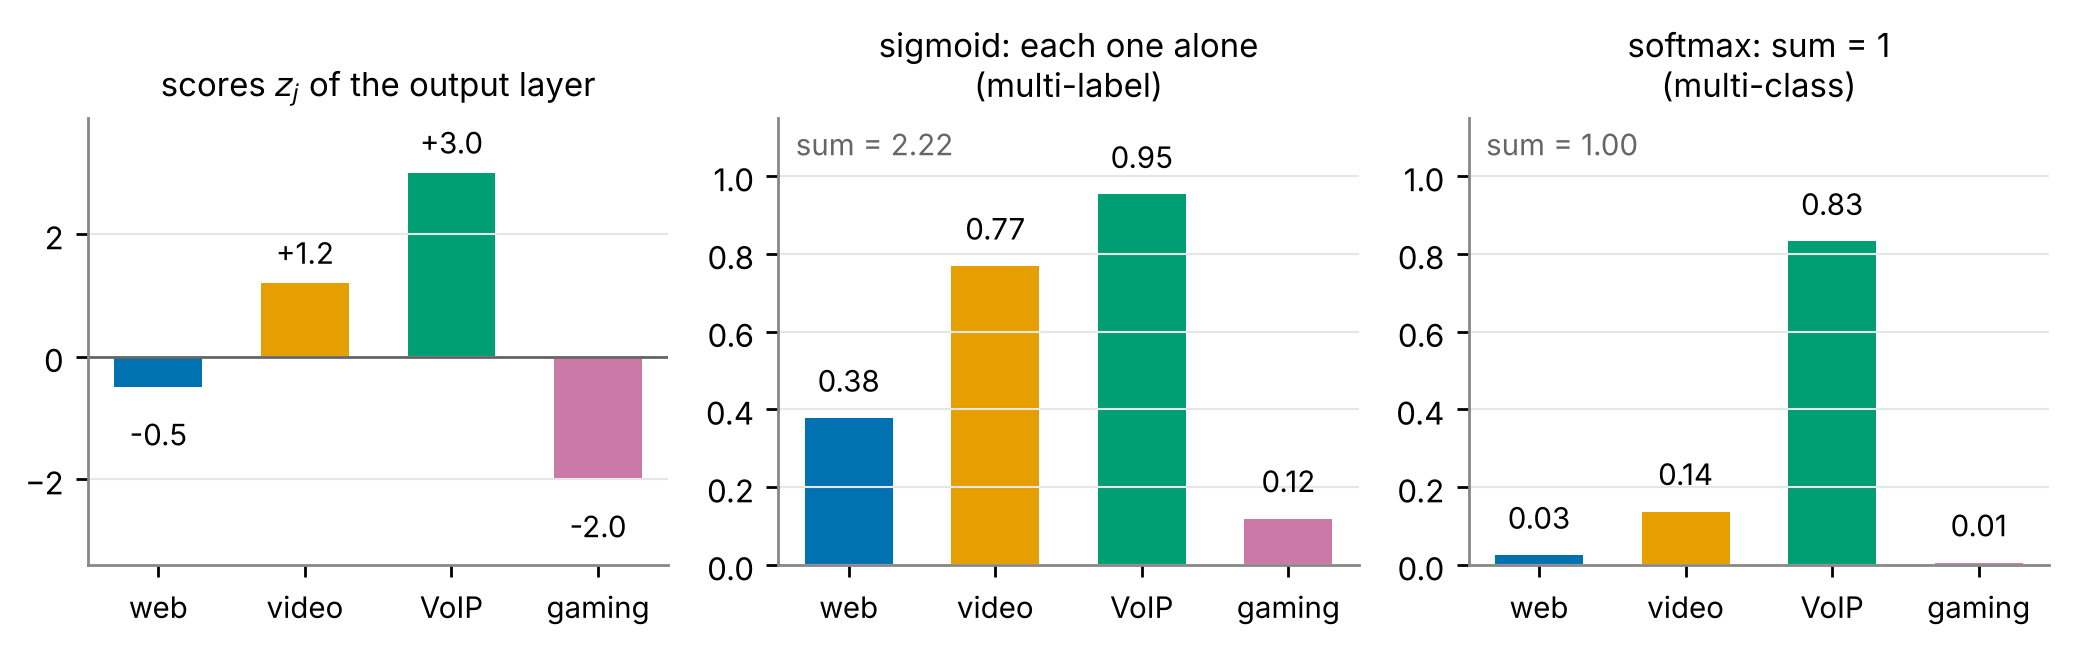
\includegraphics[width=1\textwidth]{images/chapter_11/sigmoid_softmax.png}
    \caption{The same scores of four output neurons turned into probabilities by a sigmoid on each neuron (multi-label) and by a softmax on the whole layer (multi-class).}
\end{figure}

In the figure, the scores $(-0.5, 1.2, 3, -2)$ become $(0.38, 0.77, 0.95, 0.12)$ with the sigmoid: a flow could be, at the same time, ``video'' and ``VoIP'' with high probability, and the sum is 2.22. With the softmax, $e^{z_j}$ gives $(0.61, 3.32, 20.09, 0.14)$, whose sum is $24.15$, hence the probabilities $(0.03, 0.14, 0.83, 0.01)$: a single class, VoIP, is clearly preferred.\footnote{The slides report $0.13$ for the sigmoid of $-2$ and $0.00$ for its softmax; the exact values are $0.119$ and $0.006$.}

\section{NN: Loss Function}
The most common loss function used in NNs for classification is the \textbf{cross-entropy loss}:
\[
CE = -\sum_{i=1}^{C} y_i \ln(\widehat{y}_i),
\]
where $C$ is the number of classes, $y_i$ is 1 for the true class and 0 for the others, and $\widehat{y}_i$ is the probability that the network gives to class $i$. Since only the true class has $y_i = 1$, the cross-entropy is simply $-\ln$ of the probability given to the true class: close to 0 if this probability is close to 1, very large if it is close to 0.

\paragraph{Cross-entropy with sigmoid.} With a sigmoid output there are two classes, whose labels are 0 and 1, and the network outputs a single probability $\widehat{y}$ of class 1. This is the \textbf{binary cross-entropy}:\footnote{Correction: the previous version said that with a sigmoid ``as outputs we just have 0 and 1''. It is the labels that are 0 and 1; the output of the sigmoid is a probability between 0 and 1.}
\[
CE = -y\ln(\widehat{y}) - (1-y)\ln(1-\widehat{y}) .
\]
If $y = 1$ only the first term remains, if $y = 0$ only the second one. It is the logistic loss of the Empirical Risk chapter, written for labels 0/1 instead of $\pm 1$. For a multi-label problem, the binary cross-entropy is computed for each label and summed.

\paragraph{Cross-entropy with softmax.} With a softmax output layer the same formula is used for $C$ classes, and it is called \textbf{categorical cross-entropy}:
\[
CE = -\ln\Big(\frac{e^{z_p}}{\sum_{j=1}^{C} e^{z_j}}\Big),
\]
where $z_p$ is the score of the positive (true) class.

\begin{figure}[h]
    \centering
    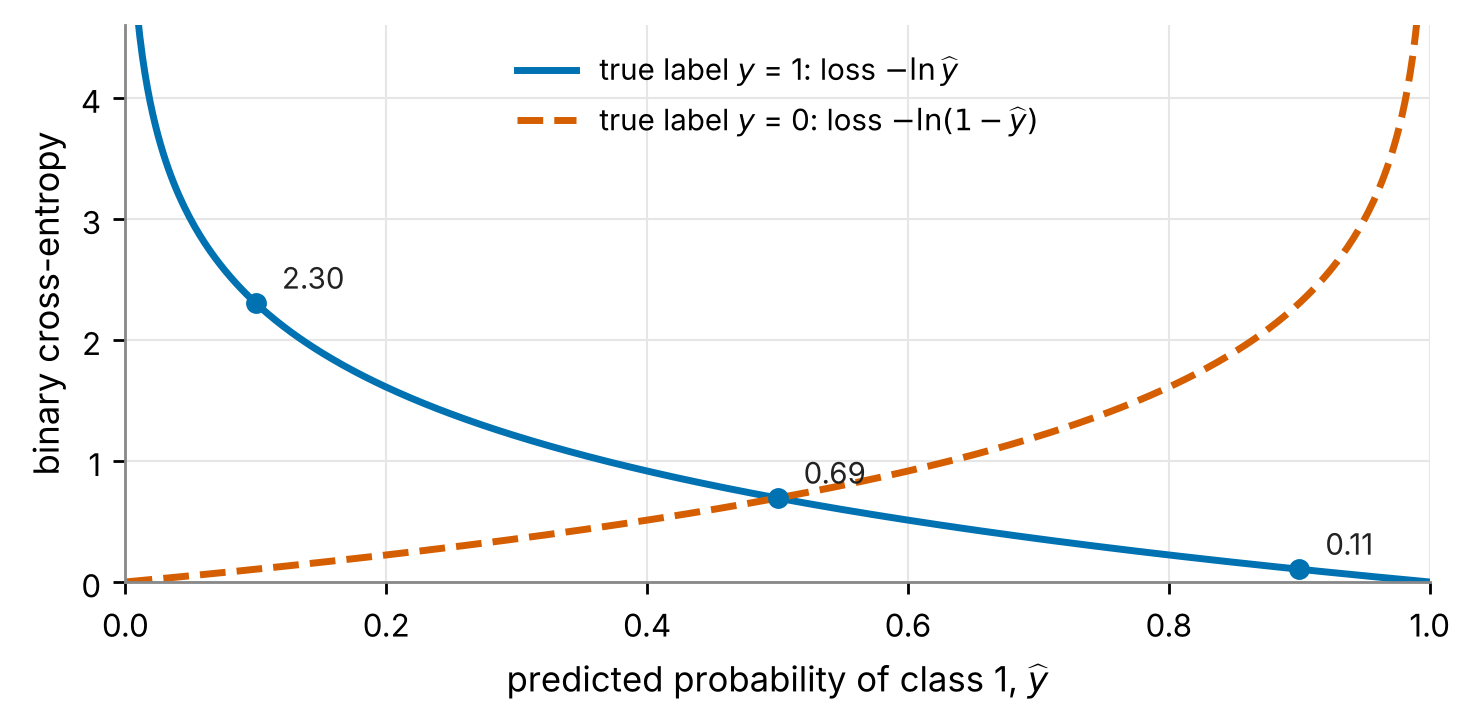
\includegraphics[width=0.75\textwidth]{images/chapter_11/cross_entropy.png}
    \caption{Binary cross-entropy as a function of the predicted probability: confident correct predictions cost almost nothing, confident wrong ones cost a lot.}
\end{figure}

For example, for a flow that is really an attack ($y = 1$), predicting $\widehat{y} = 0.9$ costs $-\ln 0.9 = 0.11$, predicting $0.5$ costs $0.69$, and predicting $0.1$ costs $2.30$. With the softmax of the previous figure, if the true class is VoIP the loss is $-\ln 0.83 = 0.18$; if it is web, which got only $0.025$, the loss is $-\ln 0.025 = 3.68$.

\section{NN: Issues}
\begin{itemize}
    \item \textbf{Long training time}: many parameters, many epochs, large datasets.
    \item \textbf{Complex configuration}: many hyperparameters to choose and tune (layers, neurons, activations, learning rate, batch size, epochs, optimizer).
    \item \textbf{Not interpretable}: a NN is a black-box model; it is hard to explain to a network operator why a flow was flagged.
    \item With many parameters and few data, NNs easily \textbf{overfit}; validation, early stopping and regularization are essential.
\end{itemize}

\section{NN: More Complex Architectures}
\paragraph{Deep NN.} Deep neural networks are NNs with many layers. They often allow to use \textbf{raw input}, with a very large number of input features, e.g. the bytes of the packets instead of features designed by hand. The multiple layers are used to progressively extract higher-level features from the raw input: the first layers find simple patterns, the following ones combine them into more abstract ones.

Two families of architectures are used for structured inputs:
\begin{itemize}
    \item for \textbf{images}, and data that can be arranged as images, \textbf{convolutional NNs} (CNN), whose neurons look at small local patches and share the same weights across the whole input. In networking, the first bytes of a flow can be arranged as a small image and classified by a CNN;
    \item for \textbf{time series}, \textbf{recurrent NNs} (RNN), whose output at each time step also depends on a state computed at the previous steps. In networking, they are used to forecast the load of a link from its recent history.
\end{itemize}

\begin{figure}[h]
    \centering
    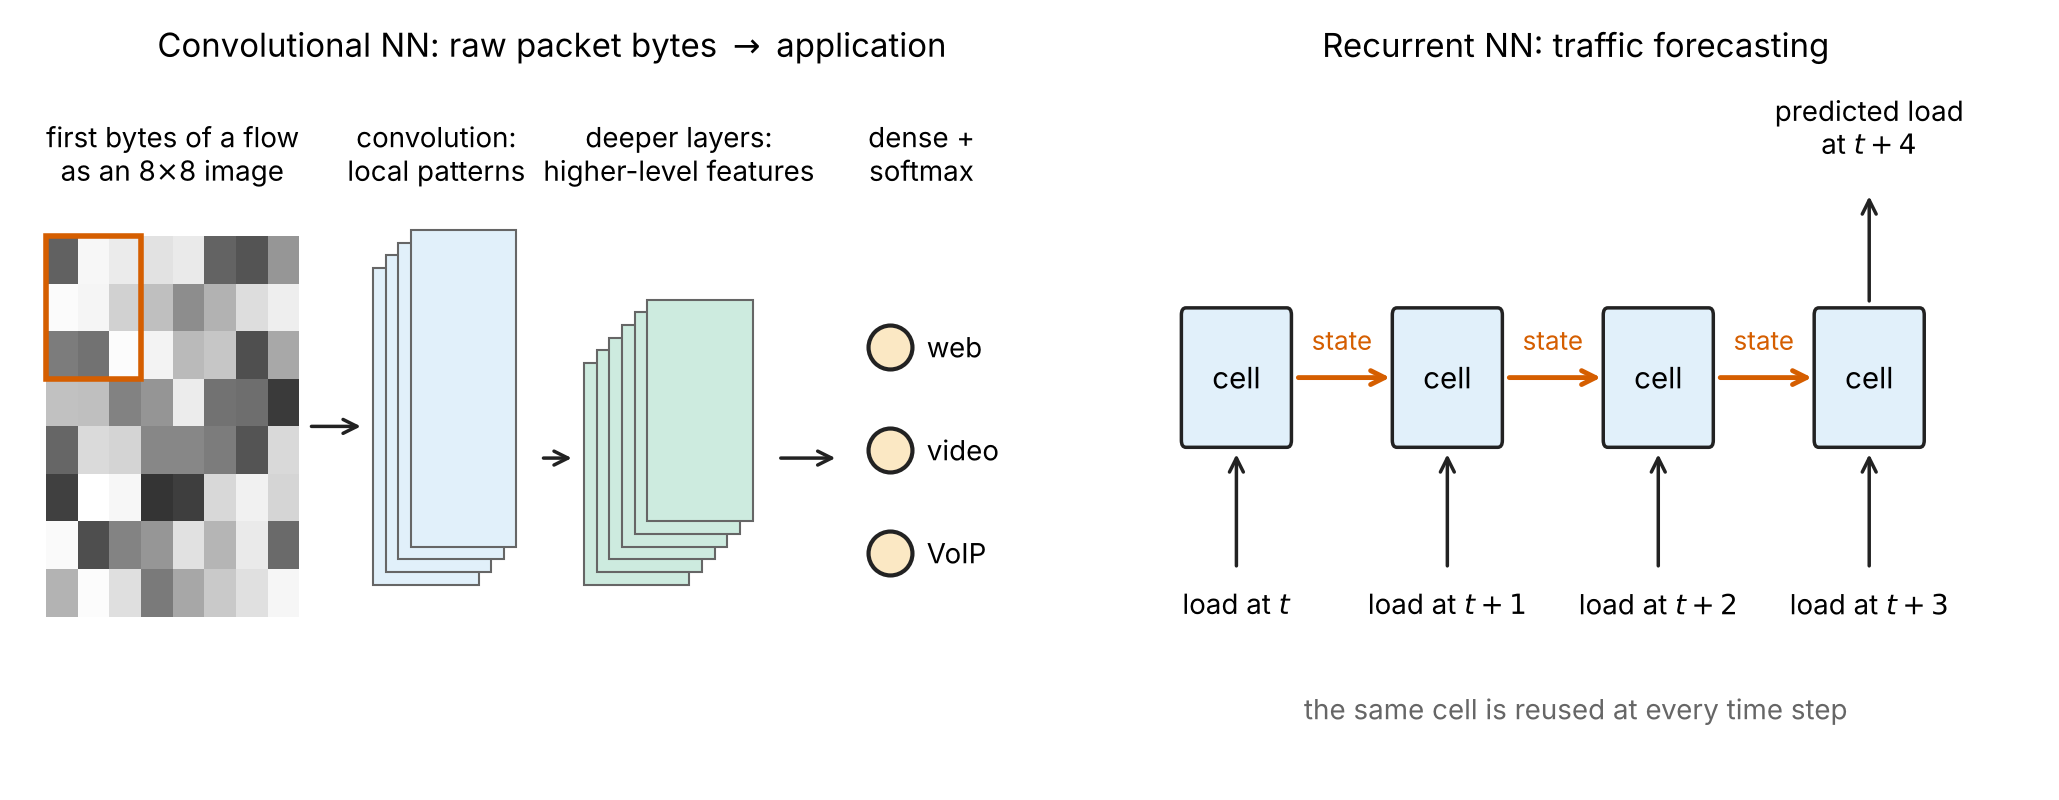
\includegraphics[width=1\textwidth]{images/chapter_11/deep_architectures.png}
    \caption{Left: a CNN classifies a flow from its first bytes. Right: an RNN, unrolled over time, forecasts the load of a link; the same cell, with the same weights, processes every time step.}
\end{figure}

\section{Self-Assessment Quiz}
\paragraph{1. Define the model (and draw the schema) of two different NNs with 3 features and 1 output, with at least one hidden layer each, and using at least two different activation functions.} Two possible answers are shown in the figure:
\begin{itemize}
    \item \textbf{NN 1}: 3 inputs, one hidden layer of 4 neurons with ReLU, 1 output neuron with sigmoid (e.g. for binary classification). Parameters: $3 \cdot 4 + 4 = 16$ for the hidden layer and $4 \cdot 1 + 1 = 5$ for the output, 21 in total.
    \item \textbf{NN 2}: 3 inputs, a hidden layer of 5 neurons with tanh, a second hidden layer of 3 neurons with ReLU, 1 output neuron without activation (e.g. for regression). Parameters: $(15 + 5) + (15 + 3) + (3 + 1) = 42$.
\end{itemize}

\begin{figure}[h]
    \centering
    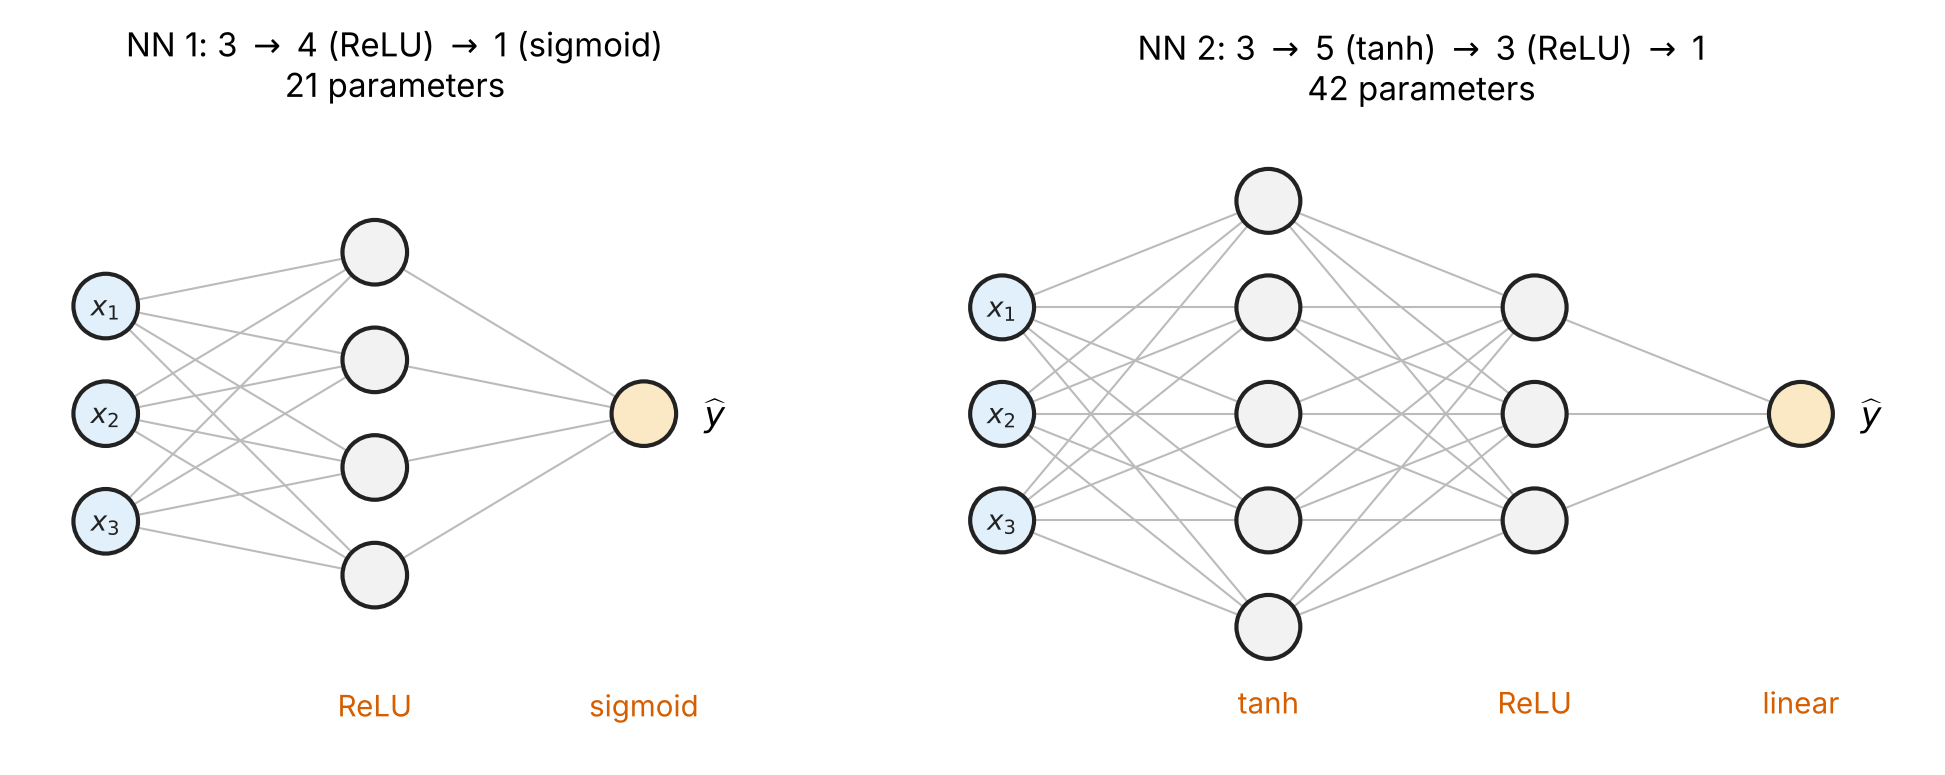
\includegraphics[width=0.95\textwidth]{images/chapter_11/quiz_networks.png}
    \caption{Two possible networks for the first question of the quiz.}
\end{figure}

\paragraph{2. Accuracy of a given NN.} The hypothesis $h$ is a single neuron with inputs $x_1$, $x_2$, weights $w_1 = 1$, $w_2 = 0$, offset $\mu = -1$ and sigmoid activation, so $\widehat{y} = \sigma(x_1 - 1)$ is the probability of class A, and the data point is assigned to class A if $\widehat{y} > 0.5$. Since $\sigma(z) > 0.5$ exactly when $z > 0$, the rule is simply ``class A if $x_1 > 1$'': $x_2$ has weight 0 and does not matter. On the dataset $D$:
\begin{center}
    \begin{tabular}{c|c|c|c|c|c}
        $x_1$ & $x_2$ & $z = x_1 - 1$ & $\widehat{y} = \sigma(z)$ & \textbf{Predicted} & \textbf{True} \\ \hline
        2  & 3  & 1  & 0.73 & A & A \\
        0  & $-4$ & $-1$ & 0.27 & B & B \\
        5  & 5  & 4  & 0.98 & A & A \\
        3  & 7  & 2  & 0.88 & A & A \\
        $-5$ & 7  & $-6$ & 0.00 & B & B \\
    \end{tabular}
\end{center}
All 5 data points are classified correctly, so the accuracy on $D$ is $5/5 = 1$. The figure shows the decision boundary $x_1 = 1$: the three points of class A lie to its right, the two of class B to its left.

\begin{figure}[H]
    \centering
    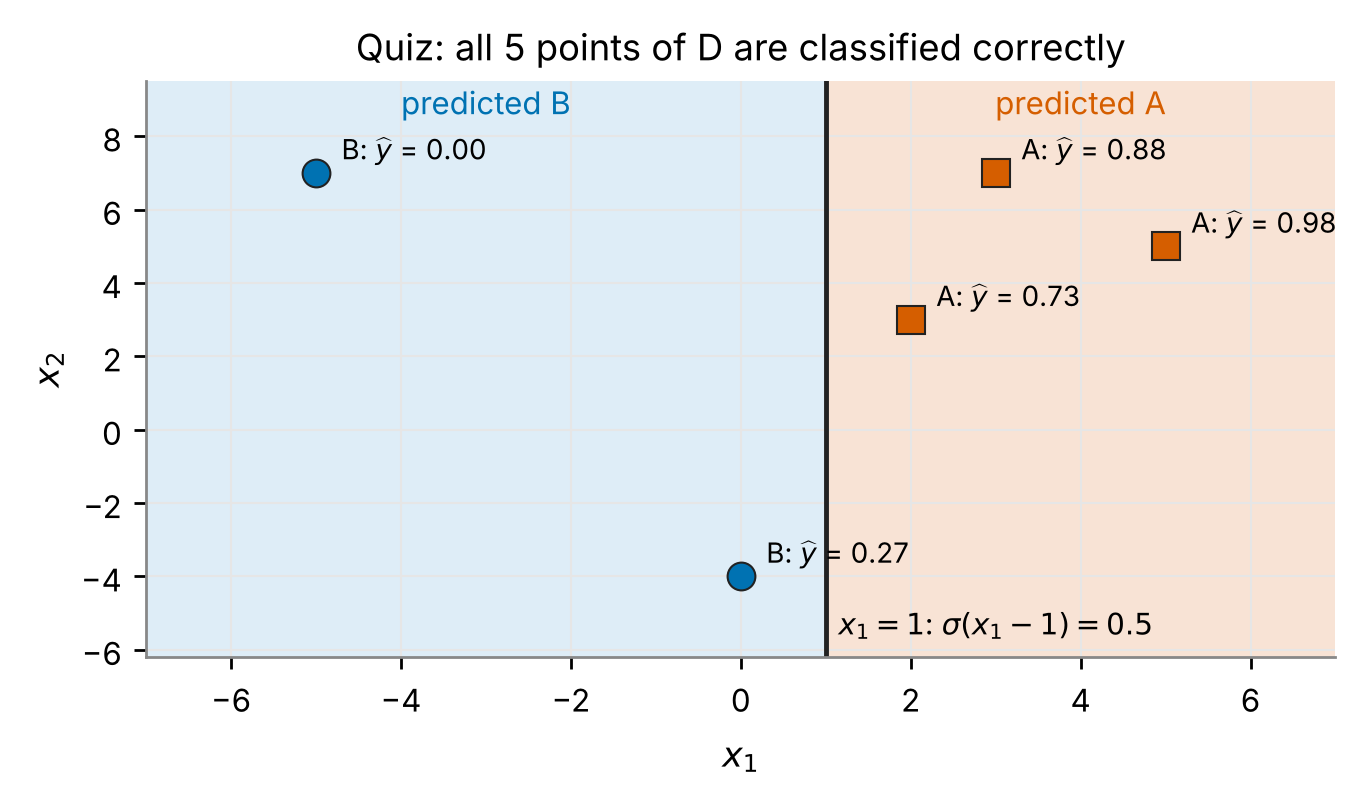
\includegraphics[width=0.5\textwidth]{images/chapter_11/quiz_boundary.png}
    \caption{The decision boundary of the quiz neuron, $x_1 = 1$, and the five points of $D$.}
\end{figure}

\section{Summary}
\begin{itemize}
    \item A NN is a model for supervised ML, trained by ERM, whose hypothesis space contains highly non-linear functions.
    \item A \textbf{neuron} computes a weighted sum of its inputs plus an offset, and applies an activation function. Linear regression is one neuron without activation, logistic regression one neuron with sigmoid.
    \item A \textbf{feed-forward NN} (MLP) stacks neurons in input, hidden and output layers. Layers, neurons and activations are hyperparameters; weights and offsets are the parameters learnt by ERM (one per connection, plus one per hidden or output neuron).
    \item Training uses \textbf{gradient descent}: the forward pass computes the prediction and the loss, the backward pass computes the gradient with the chain rule (back-propagation), and the weights are updated. Learning rate, epochs, batch size and optimizer must be chosen.
    \item Without non-linear \textbf{activation functions} the network is linear. Sigmoid, tanh, ReLU are used in hidden layers; the output layer uses sigmoid (binary or multi-label) or softmax (multi-class).
    \item The usual loss is the \textbf{cross-entropy}: binary with sigmoid, categorical with softmax.
    \item NNs are slow to train, have many hyperparameters and are black boxes. Deep NNs work on raw inputs; CNNs are used for images, RNNs for time series.
\end{itemize}



\section{A prova di coglione}
Una rete neurale non è magia: è un altro modello di ERM, solo con uno spazio di ipotesi enorme e molto flessibile. Si costruisce impilando tanti pezzi semplici, i neuroni, e si addestra con il gradient descent del capitolo 9. Nel networking serve quando le relazioni sono troppo complicate per una retta: classificare flussi, scovare anomalie, prevedere throughput e carico dei link.

\subsection{Il neurone e la rete}
\paragraph*{L'idea.} Un neurone è una piccola calcolatrice: moltiplica ogni input per un peso, somma tutto più un offset, e passa il risultato a una funzione di attivazione. Una rete è fatta di tanti neuroni in fila, a strati: le uscite di uno strato sono gli ingressi del successivo.

Esempio: con input $(-0.06, -2.5, 1.4)$, pesi $(2.7, -8.6, 0.02)$ e offset $1.1$, la somma pesata è $22.47$. Un neurone senza attivazione è la regressione lineare; con la sigmoide è la regressione logistica.

Lo strato di input ha un nodo per feature, quello di output un neurone per ogni cosa da prevedere; gli strati \textbf{nascosti} li scegli tu (quanti e quanto grandi), e sono iperparametri. I parametri, cioè pesi e offset, li impara l'ERM: uno per ogni collegamento, più un offset per ogni neurone nascosto o di uscita. Per la rete $3 \rightarrow 4 \rightarrow 3 \rightarrow 2$: $12 + 12 + 6 = 30$ pesi e $4 + 3 + 2 = 9$ offset, in tutto 39 parametri.

Perché impilare neuroni semplici dà funzioni così flessibili? Ogni neurone ReLU disegna una ``piega''; sommando abbastanza pieghe si può seguire qualunque curva, come si costruisce una curva con tanti pezzetti di righello.

\begin{figure}[h]
    \centering
    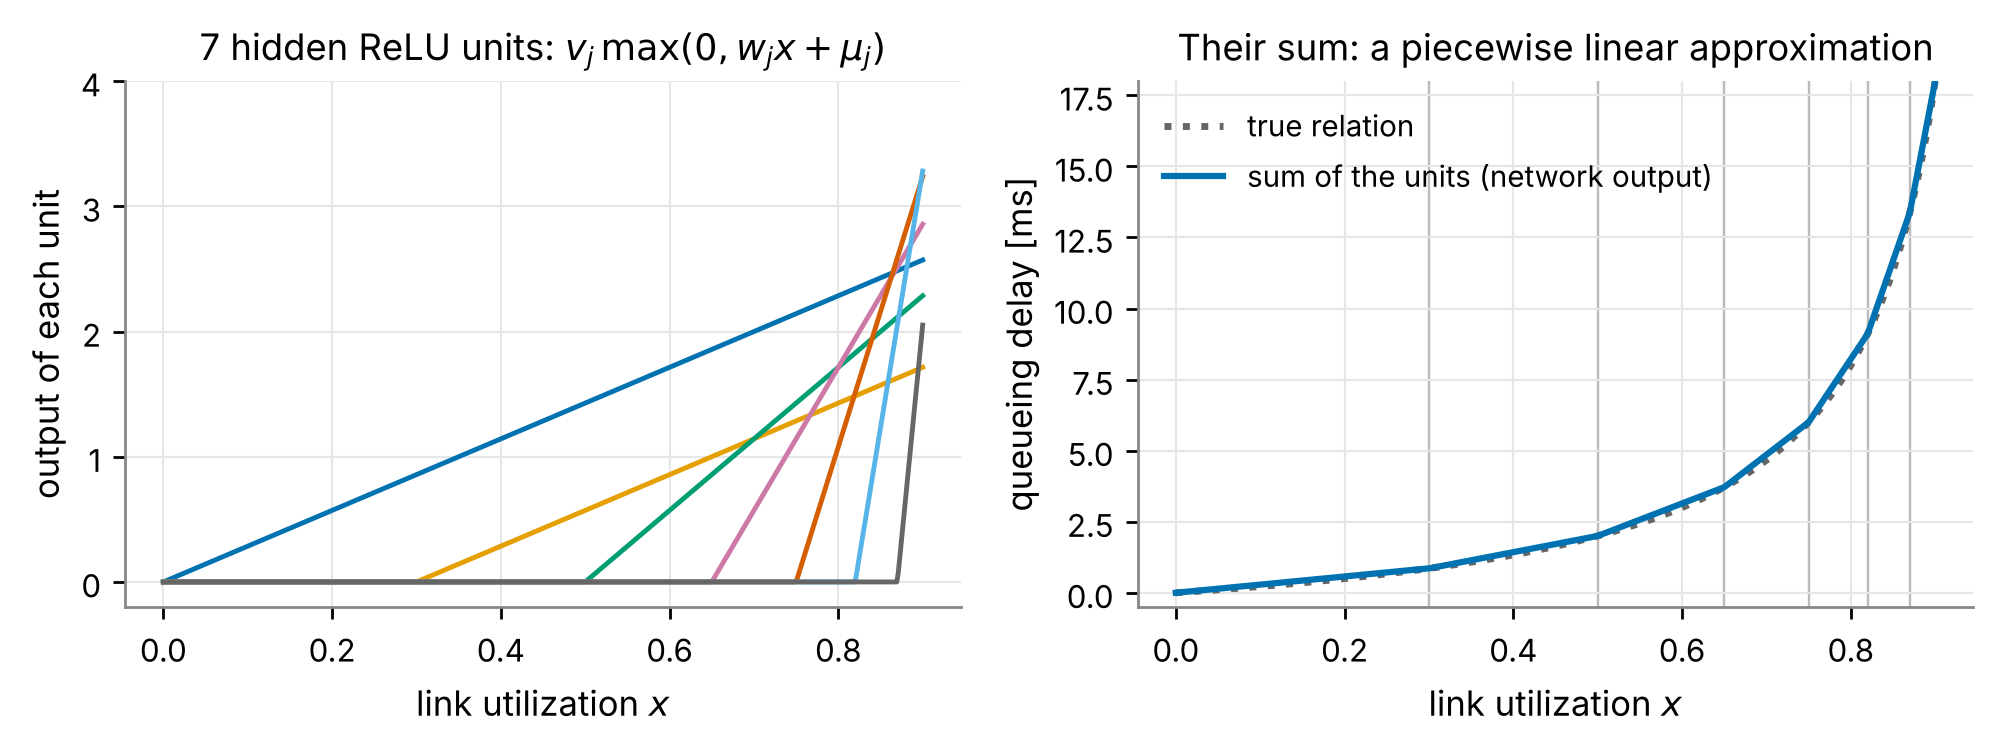
\includegraphics[width=0.85\textwidth]{images/chapter_11/relu_sum.png}
    \caption{Sette neuroni ReLU, ognuno una piega; la loro somma segue la curva del ritardo del link.}
\end{figure}

\subsection{Le funzioni di attivazione}
\paragraph*{L'idea.} Senza attivazione, una rete con cento strati fa esattamente quello che fa una retta: una mappa lineare di una mappa lineare resta lineare. È l'attivazione \emph{non lineare} a dare alla rete la capacità di piegarsi.

Nel capitolo: la stessa rete su due classi a cerchi concentrici arriva al 65\% senza attivazione e al 100\% con ReLU. Negli strati nascosti si usano ReLU (la scelta di default), tanh o sigmoide; il gradino non si usa, perché la sua derivata è zero e il gradient descent non saprebbe dove andare.

In uscita la scelta dipende dal problema. Regressione: nessuna attivazione. Binaria: una sigmoide. Multi-class: softmax, che trasforma i punteggi in probabilità con somma 1. Multi-label: una sigmoide per ogni etichetta, perché ogni etichetta è una domanda sì/no a sé. Esempio: i punteggi $(-0.5, 1.2, 3, -2)$ diventano $(0.03, 0.14, 0.83, 0.01)$ con la softmax.

\subsection{Come impara: forward, backward, update}
\paragraph*{L'idea.} La rete fa una previsione (forward), misura quanto ha sbagliato (loss), capisce di chi è la colpa risalendo all'indietro strato per strato (backward), e corregge ogni peso di un passettino (update). Si ripete finché la loss non scende più.

La loss è una sola, calcolata in uscita. La backpropagation distribuisce la ``colpa'' a ogni peso con la regola della catena: la derivata della loss rispetto a un peso è il prodotto delle derivate locali lungo il percorso. Per un neurone sigmoide con cross-entropy il risultato è sorprendentemente semplice: gradiente $= (\widehat{y} - y)\,x$, cioè errore per input. Esempio: $x = 2$, $w = 0.5$, $y = 1$: la previsione è $0.731$, il gradiente $-0.538$, e con $\alpha = 0.5$ il peso passa a $0.769$ e la loss scende da $0.313$ a $0.195$.

Gli iperparametri dell'addestramento sono il learning rate, il numero di epoche (un'epoca è un passaggio completo sui dati, non un singolo aggiornamento), la dimensione del batch e l'ottimizzatore. Con 10\,000 flussi e batch da 100, un'epoca sono 100 aggiornamenti.

\begin{figure}[h]
    \centering
    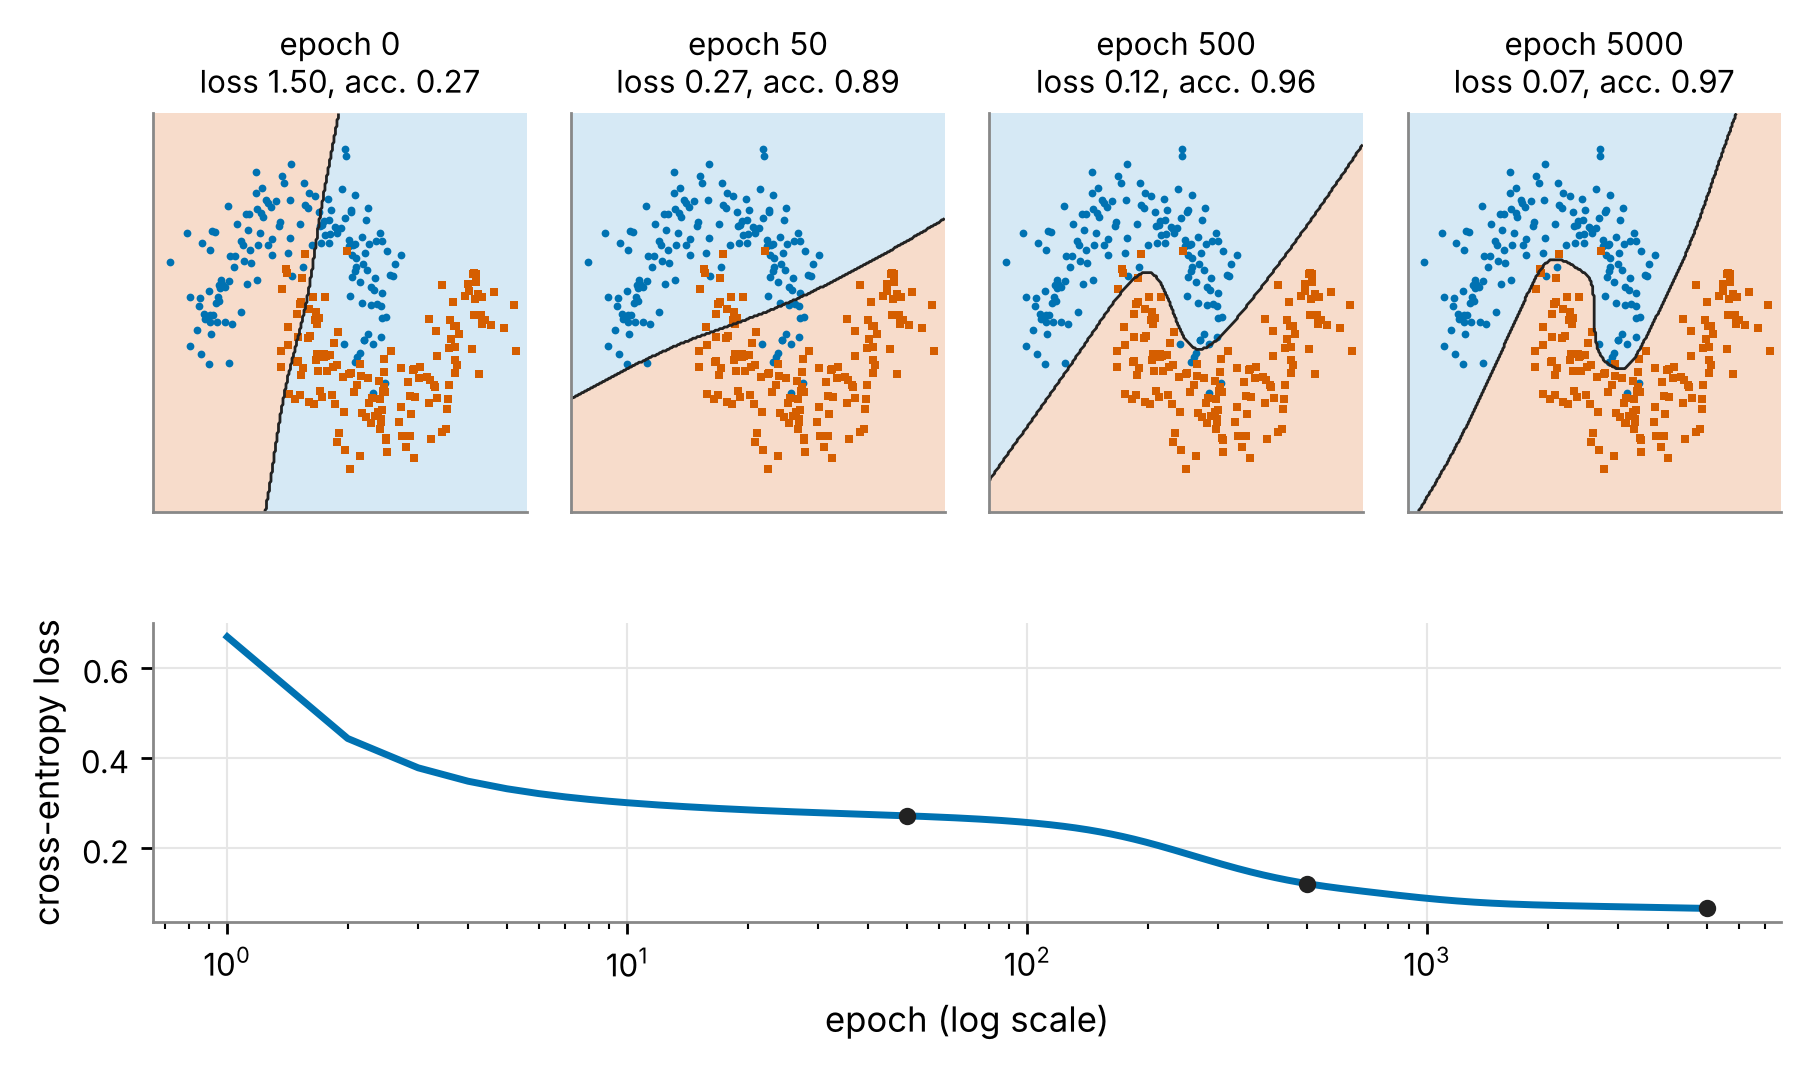
\includegraphics[width=0.85\textwidth]{images/chapter_11/training_evolution.png}
    \caption{All'inizio i pesi sono casuali e il confine pure; epoca dopo epoca la loss scende e il confine si piega attorno alle classi.}
\end{figure}

\subsection{La loss: cross-entropy}
\paragraph*{L'idea.} La cross-entropy è $-\ln$ della probabilità data alla classe giusta. Se la rete è sicura e ha ragione costa quasi zero; se è sicura e ha torto costa tantissimo.

Per un attacco vero ($y = 1$): prevedere $0.9$ costa $0.11$, prevedere $0.5$ costa $0.69$, prevedere $0.1$ costa $2.30$. Con la sigmoide si chiama \emph{binary} cross-entropy (le label sono 0 e 1, l'uscita è una probabilità), con la softmax \emph{categorical} cross-entropy.

\subsection{Pregi, difetti e reti profonde}
Le reti sono flessibilissime, ma sono lente da addestrare, hanno tanti iperparametri e sono scatole nere, cioè è difficile spiegare perché hanno deciso qualcosa. Le reti profonde (deep) hanno molti strati e possono lavorare sui dati grezzi: le CNN su dati organizzati come immagini (anche i byte di un pacchetto), le RNN su serie temporali (il carico di un link nel tempo).

\paragraph*{Il quiz.} La rete del quiz è un solo neurone che calcola $\sigma(x_1 - 1)$: dice A quando $x_1 > 1$, e $x_2$ non conta perché ha peso 0. Sui 5 punti di D non sbaglia mai: accuratezza 1.

\subsection{Da sapere per l'esame}
\begin{center}
    \begin{tabular}{l|l}
        \textbf{Concetto} & \textbf{In una riga} \\ \hline
        Neurone            & $\widehat{y} = \sigma(w_1x_1 + \dots + w_nx_n + \mu)$ \\ \hline
        Casi particolari   & 1 neurone lineare: regr. lineare; con sigmoide: logistica \\ \hline
        MLP                & strati input, nascosti, output; layer densi \\ \hline
        Iperparametri      & numero di strati, neuroni per strato, attivazioni \\ \hline
        Parametri          & pesi (uno per connessione) + offset (no input) \\ \hline
        Forward pass       & dagli input alla previsione e alla loss \\ \hline
        Backward pass      & gradiente con la regola della catena, a ritroso \\ \hline
        Neurone sigmoide   & $\partial L/\partial w = (\widehat{y} - y)\,x$ con la cross-entropy \\ \hline
        Epoca              & un passaggio sui dati: $m/B$ aggiornamenti \\ \hline
        Senza attivazione  & la rete resta lineare, qualunque sia la profondità \\ \hline
        Uscita             & lineare, sigmoide (binaria) o softmax (multi-class) \\ \hline
        Softmax            & $e^{z_j}/\sum_i e^{z_i}$: probabilità con somma 1 \\ \hline
        Cross-entropy      & $-\ln$(probabilità della classe vera) \\ \hline
        Difetti            & training lento, tanti iperparametri, scatola nera \\ \hline
        Deep               & tanti strati, input grezzi; CNN e RNN \\
    \end{tabular}
\end{center}
